

\subsection{Clusters}\label{sec:result:clusters}

\Warning[TODO]{ Rewrite this section! }

This is a simple clustering analysis of the datasets, clustered on a user basis.

The clustering algorithm used is k-means, operating on $U * S$ if $U * S * V'$ forms a rank $k$ SVD approximation of the interaction matrix $A$. The resulting rows in the matrix (the user ones) are then reordered and grouped with respect to their clusters.

This will try to group similar users next to each other. The used number of clusters is 10, this is not the optimal number of clusters for the datasets but the results are still useful for determining if there exists any clusters in the datasets.

Some of the graphs will be sparse and some will appear to be very dense. This is mostly due to resolution issues as when the dataset grow, even though the sparsity might be lower, the number of data points grow but the size of each data point in the graphs are the same.

\FloatBarrier

\twopic{fig/data/alphaS_original.png}{fig/data/alphaS_10-clusters.png}{
\textit{alphaS}
}

In \textit{alphaS} there are some clusters whith relatively few item interactions, but the other clusters aren't very prominent. Both \textit{alpha} and \textit{alpha2} are so large the resolution isn't enough to capture any individual data points so their graphs doesn't show anything of value so they are not included here.

\twopic{fig/data/eswc2015books_original.png}{fig/data/eswc2015books_10-clusters.png}{
\textit{eswc2015books}
}

\FloatBarrier

\textit{eswc2015books} doesn't seem to have any major clusters, the dataset doesn't appear to have any structure except for a few streaks of very popular items.

\FloatBarrier

\twopic{fig/data/eswc2015movies_original.png}{fig/data/eswc2015movies_10-clusters.png}{
\textit{eswc2015movies}
}

\twopic{fig/data/eswc2015music_original.png}{fig/data/eswc2015music_10-clusters.png}{
\textit{eswc2015music}
}

\textit{eswc2015movies} and \textit{eswc2015music} in contrast display more prominent clusters. There are clusters who concentrate more on a subset of items, and there are clusters with higher interaction count.  Similarly \textit{movielens1m} and \textit{romeo} also have distinct clusters.

\twopic{fig/data/movielens1m_original.png}{fig/data/movielens1m_10-clusters.png}{
\textit{movielens1m}
}

\twopic{fig/data/romeo_original.png}{fig/data/romeo_10-clusters.png}{
\textit{romeo}
}

\FloatBarrier

\twodiffpic{fig/data/alphaS_10-clusters_item_sorted.png}{\textit{alphaS}}
{fig/data/eswc2015books_10-clusters_item_sorted.png}{\textit{eswc2015books}}

\twodiffpic{fig/data/eswc2015movies_10-clusters_item_sorted.png}{\textit{eswc2015movies}}
{fig/data/eswc2015music_10-clusters_item_sorted.png}{\textit{eswc2015music}}

\twodiffpic{fig/data/movielens1m_10-clusters_item_sorted.png}{\textit{movielens1m}}
{fig/data/romeo_10-clusters_item_sorted.png}{\textit{romeo}}

\FloatBarrier

\newpage

\subsection{Spectral clustering}

k-means cluster for compactness while spectral clustering cluster based on connectivity.

\url{https://charlesmartin14.wordpress.com/2012/10/09/spectral-clustering/}

The basic steps are as follows:

\begin{enumerate}
    \item Create an affinity matrix, or simpler an adjacency matrix, $A_{f}$
    \item Construct a Graph Laplacian $L$
    \item Find eigenvalues and eigenvectors of $L$
    \item Select a subspace of eigenvectors
    \item Form clusters in the subspace
\end{enumerate}

In our particular case, the interaction matrix $A$ is defined as rows corresponding to users and columns corresponding to items. The affinity matrix needs to be square, but the interaction matrix is not. There are other more complex ways of creating an affinity matrix, but for this purpose modelling a simple adjacency matrix is sufficient.
\Warning[TODO]{ What complex ways? }

A transformation from the interaction matrix $A$ to the adjacency matrix $A_{f}$ is made by having both users and items as both row and column indices and mirroring the interactions. $A_{f}$ will then be a symmetric, square matrix. \eqref{eq:make_adj} illustrates an example.

\begin{equation}\label{eq:make_adj}
  A = \kbordermatrix{
    &    i_1 & i_2 & i_3 & i_4 \\
    u_1 & 0   & 1   & 0   & 1  \\
    u_2 & 0   & 1   & 1   & 1  \\
    u_3 & 1   & 0   & 1   & 0
  }
  \Rightarrow
    A_f = \kbordermatrix{
        &    u_1 & u_2 & u_3 & i_1 & i_2 & i_3 & i_4 \\
        u_1 & 0   & 0   & 0  &  0  &  1  &  0  &  1  \\
        u_2 & 0   & 0   & 0  &  0  &  1  &  1  &  1  \\
        u_3 & 0   & 0   & 0  &  1  &  0  &  1  &  0 \\
        i_1 & 0   & 0   & 1  &  0  &  0  &  0  &  0 \\
        i_2 & 1   & 1   & 0  &  0  &  0  &  0  &  0 \\
        i_3 & 0   & 1   & 1  &  0  &  0  &  0  &  0 \\
        i_4 & 1   & 1   & 0  &  0  &  0  &  0  &  0 \\
    }
\end{equation}

\begin{figure}[h!]
    \centering
    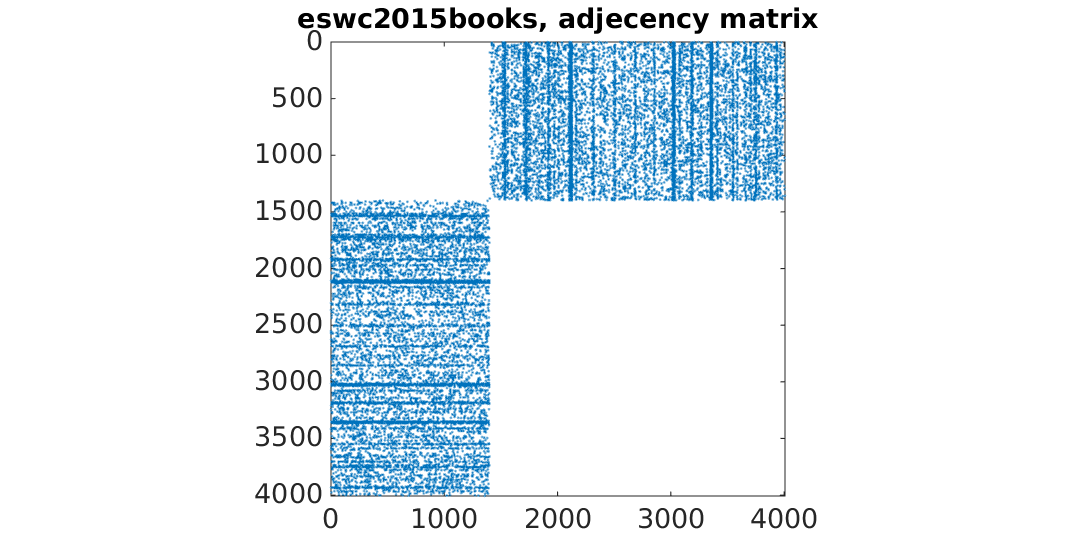
\includegraphics[width=0.3\linewidth]{fig/spectral_data/eswc2015books_adj.png}
    \caption{Adjacency matrix for \textit{eswc2015books}}
    %\label{fig:ex_graph_link_rec}
\end{figure}

There are different kinds of Laplacians in literature, the one used here is the simple Laplacian $L = D - A_f$ where $D$ is a diagonal matrix called the degree matrix, representing the sum of the degrees at each node $i$:
\Warning[TODO]{ Ref needed! }

\begin{equation}
    D_{i, i} = \sum_j a_{i, j}
\end{equation}

The principal idea is that if good clusters can be identified, then the Laplacian $L$ is approximately block diagonal, with each cluster defined by a block. That is if there are 3 clusters

\begin{equation}
    \begin{pmatrix}
        L_{1, 1} & L_{1, 2} & L_{1, 3} \\
        L_{2, 1} & L_{2, 2} & L_{2, 3} \\
        L_{3, 1} & L_{3, 2} & L_{3, 3}
    \end{pmatrix}
    \sim
    \begin{pmatrix}
        L_{1, 1} & 0         & 0         \\
        0        & L_{2, 2} & 0      \\
        0        & 0         & L_{3, 3}
    \end{pmatrix}
\end{equation}

Then also the lowest eigenvalues and eigenvectors correspond...

\twodiffpic{fig/spectral_data/eswc2015books_eig_sort.png}
{Sorted by sorting the 2nd eigenvector}
{fig/spectral_data/eswc2015books_kmeans_sort.png}
{Sorted by k-means clustering of the 2nd eigenvector}

%/fig/spectral_data 
%eswc2015books_adj.png

%eswc2015books_eig_sort.png
%eswc2015books_eigv.png
%eswc2015books_kmeans_sort.png
%eswc2015books_spectral_clust.png

\twodiffpic{fig/spectral_data/eswc2015books_eigv.png}
{The smallest eigenvalues}
{fig/spectral_data/eswc2015books_spectral_clust.png}
{Original matrix sorted using spectral clustering}

